\documentclass[border=1]{standalone}
\usepackage{xcolor}
\usepackage{tikz}

\definecolor{magenta}{HTML}{f8766d}
\definecolor{cyan}{HTML}{00bfc4}
\usetikzlibrary{arrows, arrows.meta, patterns}

\tikzset{
    point/.style={ draw, scale=0.25, color=blue, circle, fill },
    cell/.style={draw, dashed},
    p1/.style={solid, fill=magenta!15},
    %p2/.style={solid,pattern color=cyan!75, pattern={north east lines}},
    p2/.style={solid, fill=cyan!15},
    line/.style={ % style that just defines the arrow tip
        >={Triangle[left,length=5pt,width=5pt]},
        double,
        <->
    },
    whites/.style={
        thick, 
        color=white
    }
}

\begin{document}
    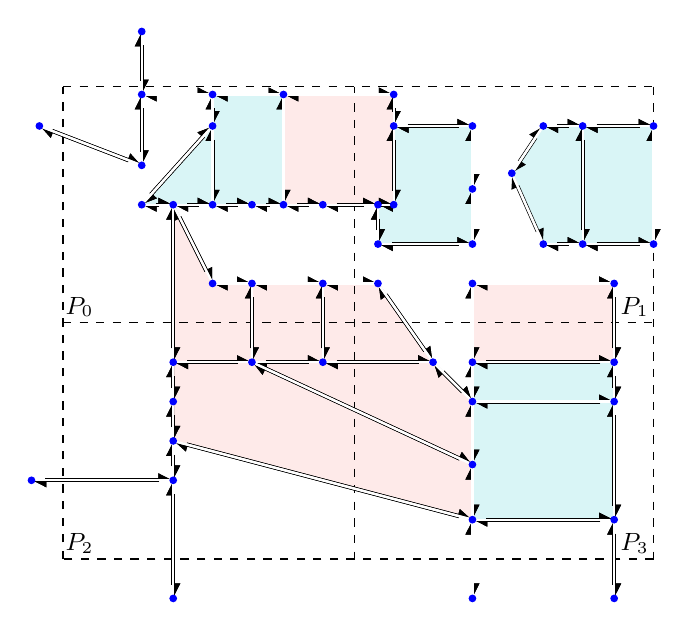
\begin{tikzpicture}
        \draw[p1] (2.7934, 5.9017) -- (2.7934, 4.5017) -- (4.1934, 4.5017) -- (4.1934, 5.9017) -- (2.7934, 5.9017) -- cycle;
\draw[p1] (1.3934, 4.5017) -- (1.3934, 1.5017) -- (5.1934, 0.5016) -- (5.1934, 2.0017) -- (4.6934, 2.5017) -- (3.9934, 3.5017) -- (1.8934, 
3.5017) -- (1.3934, 4.5017) -- cycle;
\draw[p1] (5.1934, 3.5017) -- (5.1934, 2.5017) -- (6.9934, 2.5017) -- (6.9934, 3.5017) -- (5.1934, 3.5017) -- cycle;

        \draw[p2] (1.893, 5.502) -- (0.993, 4.502) -- (2.793, 4.502) -- (2.793, 5.902) -- (1.893, 5.902) -- (1.893, 5.502) -- cycle;
\draw[p2] (4.193, 5.502) -- (4.193, 4.502) -- (3.993, 4.502) -- (3.993, 4.002) -- (5.193, 4.002) -- (5.193, 5.502) -- (4.193, 5.502) -- cycle;
\draw[p2] (6.093, 5.502) -- (5.693, 4.902) -- (6.093, 4.002) -- (7.493, 4.002) -- (7.493, 5.502) -- (6.093, 5.502) -- cycle;
\draw[p2] (5.193, 2.502) -- (5.193, 0.502) -- (6.993, 0.502) -- (6.993, 2.502) -- (5.193, 2.502) -- cycle;

        \draw[cell] (-0.01, 6.0) -- (7.49, 6.0);
\draw[cell] (7.49, 6.0) -- (7.49, 0.0);
\draw[cell] (7.49, 0.0) -- (-0.01, 0.0);
\draw[cell] (-0.01, 0.0) -- (-0.01, 6.0);
\draw[cell] (-0.01, 3.0) -- (7.49, 3.0);
\draw[cell] (3.69, 6.0) -- (3.69, 0.0);
\node[] at (0.2,3.2) {\small $P_0$};
\node[] at (7.25,3.2) {\small $P_1$};
\node[] at (0.2,0.2) {\small $P_2$};
\node[] at (7.25,0.2) {\small $P_3$};


        \draw[line] (-0.31, 5.5) -- (0.99, 5.0);
\draw[line] (0.99, 5.0) -- (0.99, 5.9);
\draw[line] (0.99, 5.9) -- (0.99, 6.7);
%\draw[line] (0.49, 4.0) -- (0.49, 4.5);
%\draw[line] (0.49, 4.5) -- (0.99, 4.5);
\draw[line] (0.99, 4.5) -- (1.89, 5.5);
\draw[line] (0.99, 5.9) -- (1.89, 5.9);
\draw[line] (1.89, 5.9) -- (2.79, 5.9);
\draw[line] (2.79, 5.9) -- (4.19, 5.9);
\draw[line] (1.89, 5.9) -- (1.89, 5.5);
\draw[line] (1.89, 5.5) -- (1.89, 4.5);
\draw[line] (0.99, 4.5) -- (1.39, 4.5);
\draw[line] (1.39, 4.5) -- (1.89, 4.5);
\draw[line] (1.39, 4.5) -- (1.39, 2.5);
\draw[line] (1.39, 2.5) -- (1.39, 2.0);
\draw[line] (1.39, 2.0) -- (1.39, 1.5);
\draw[line] (1.39, 1.5) -- (1.39, 1.0);
\draw[line] (1.39, 1.0) -- (1.39, -0.5);
\draw[line] (1.39, 1.0) -- (-0.41, 1.0);
%\draw[line] (1.39, 1.5) -- (0.49, 1.5);
%\draw[line] (1.39, 2.0) -- (0.49, 2.0);
\draw[line] (1.89, 4.5) -- (2.39, 4.5);
\draw[line] (2.39, 4.5) -- (2.79, 4.5);
\draw[line] (2.79, 4.5) -- (2.79, 5.9);
\draw[line] (2.79, 4.5) -- (3.29, 4.5);
\draw[line] (3.29, 4.5) -- (3.99, 4.5);
%\draw[line] (3.29, 4.5) -- (3.29, 3.9);
%\draw[line] (2.79, 4.5) -- (2.79, 3.9);
%\draw[line] (2.39, 4.5) -- (2.39, 3.9);
\draw[line] (2.39, 3.5) -- (2.39, 2.5);
\draw[line] (1.39, 2.5) -- (2.39, 2.5);
\draw[line] (2.39, 2.5) -- (3.29, 2.5);
\draw[line] (2.39, 3.5) -- (3.29, 3.5);
\draw[line] (1.89, 3.5) -- (2.39, 3.5);
\draw[line] (1.39, 4.5) -- (1.89, 3.5);
\draw[line] (3.29, 3.5) -- (3.99, 3.5);
\draw[line] (3.29, 2.5) -- (4.69, 2.5);
\draw[line] (3.29, 3.5) -- (3.29, 2.5);
\draw[line] (2.39, 2.5) -- (5.19, 1.2);
\draw[line] (1.39, 1.5) -- (5.19, 0.5);
\draw[line] (5.19, 0.5) -- (5.19, -0.5);
\draw[line] (5.19, 1.2) -- (5.19, 0.5);
\draw[line] (5.19, 2.0) -- (5.19, 1.2);
\draw[line] (5.19, 2.5) -- (5.19, 2.0);
\draw[line] (4.69, 2.5) -- (5.19, 2.0);
\draw[line] (3.99, 3.5) -- (4.69, 2.5);
%\draw[line] (3.99, 3.5) -- (4.69, 3.5);
\draw[line] (4.19, 5.9) -- (4.19, 5.5);
\draw[line] (4.19, 5.5) -- (5.19, 5.5);
\draw[line] (4.19, 5.5) -- (4.19, 4.5);
\draw[line] (5.19, 5.5) -- (5.19, 4.7);
\draw[line] (5.19, 4.7) -- (5.19, 4.0);
\draw[line] (3.99, 4.0) -- (5.19, 4.0);
\draw[line] (3.99, 4.5) -- (3.99, 4.0);
%\draw[line] (5.19, 4.7) -- (5.69, 4.9);
%\draw[line] (5.69, 4.9) -- (6.09, 5.0);
\draw[line] (5.69, 4.9) -- (6.09, 5.5);
%\draw[line] (5.69, 4.9) -- (6.09, 4.0);
\draw[line] (6.09, 4.0) -- (6.59, 4.0);
\draw[line] (6.09, 5.5) -- (6.59, 5.5);
\draw[line] (6.59, 5.5) -- (6.59, 4.0);
\draw[line] (6.59, 5.5) -- (7.49, 5.5);
\draw[line] (7.49, 5.5) -- (7.49, 4.0);
\draw[line] (6.59, 4.0) -- (7.49, 4.0);
\draw[line] (5.19, 3.5) -- (6.99, 3.5);
\draw[line] (5.19, 3.5) -- (5.19, 2.5);
\draw[line] (5.19, 2.5) -- (6.99, 2.5);
\draw[line] (5.19, 2.0) -- (6.99, 2.0);
\draw[line] (5.19, 0.5) -- (6.99, 0.5);
\draw[line] (6.99, 3.5) -- (6.99, 2.5);
\draw[line] (6.99, 2.5) -- (6.99, 2.0);
\draw[line] (6.99, 2.0) -- (6.99, 0.5);
\draw[line] (6.99, 0.5) -- (6.99, -0.5);
\draw[line] (3.99, 4.5) -- (4.19, 4.5);
\draw[line] (0.99, 5.0) -- (-0.31, 5.5);
\draw[line] (0.99, 5.9) -- (0.99, 5.0);
%\draw[line] (0.49, 4.5) -- (0.49, 4.0);
%\draw[line] (0.49, 2.0) -- (1.39, 2.0);
%\draw[line] (0.49, 1.5) -- (1.39, 1.5);
\draw[line] (-0.41, 1.0) -- (1.39, 1.0);
\draw[line] (1.39, -0.5) -- (1.39, 1.0);
\draw[line] (1.39, 1.0) -- (1.39, 1.5);
\draw[line] (1.39, 1.5) -- (1.39, 2.0);
\draw[line] (1.39, 2.0) -- (1.39, 2.5);
\draw[line] (2.39, 2.5) -- (1.39, 2.5);
\draw[line] (3.29, 2.5) -- (2.39, 2.5);
\draw[line] (5.19, 1.2) -- (2.39, 2.5);
\draw[line] (5.19, 0.5) -- (1.39, 1.5);
\draw[line] (2.39, 3.5) -- (1.89, 3.5);
\draw[line] (2.39, 2.5) -- (2.39, 3.5);
\draw[line] (3.29, 3.5) -- (2.39, 3.5);
\draw[line] (3.29, 2.5) -- (3.29, 3.5);
\draw[line] (3.99, 3.5) -- (3.29, 3.5);
\draw[line] (4.69, 2.5) -- (3.29, 2.5);
\draw[line] (4.69, 2.5) -- (3.99, 3.5);
%\draw[line] (4.69, 3.5) -- (3.99, 3.5);
%\draw[line] (3.29, 3.9) -- (3.29, 4.5);
%\draw[line] (2.79, 3.9) -- (2.79, 4.5);
%\draw[line] (2.39, 3.9) -- (2.39, 4.5);
\draw[line] (1.89, 4.5) -- (1.89, 5.5);
\draw[line] (1.89, 5.5) -- (0.99, 4.5);
\draw[line] (1.39, 4.5) -- (0.99, 4.5);
%\draw[line] (0.99, 4.5) -- (0.49, 4.5);
\draw[line] (1.89, 4.5) -- (1.39, 4.5);
\draw[line] (2.39, 4.5) -- (1.89, 4.5);
\draw[line] (2.79, 4.5) -- (2.39, 4.5);
\draw[line] (3.29, 4.5) -- (2.79, 4.5);
\draw[line] (3.99, 4.5) -- (3.29, 4.5);
\draw[line] (3.99, 4.0) -- (3.99, 4.5);
\draw[line] (4.19, 4.5) -- (3.99, 4.5);
\draw[line] (4.19, 4.5) -- (4.19, 5.5);
\draw[line] (5.19, 5.5) -- (4.19, 5.5);
\draw[line] (5.19, 4.0) -- (5.19, 4.7);
\draw[line] (5.19, 4.7) -- (5.19, 5.5);
\draw[line] (5.19, 4.0) -- (3.99, 4.0);
\draw[line] (6.09, 4.0) -- (5.69, 4.9);
%\draw[line] (5.69, 4.9) -- (5.19, 4.7);
%\draw[line] (6.09, 5.0) -- (5.69, 4.9);
%\draw[line] (6.09, 5.5) -- (5.69, 4.9);
\draw[line] (6.59, 5.5) -- (6.09, 5.5);
\draw[line] (6.59, 4.0) -- (6.59, 5.5);
\draw[line] (6.59, 4.0) -- (6.09, 4.0);
\draw[line] (1.39, 2.5) -- (1.39, 4.5);
\draw[line] (5.19, 2.0) -- (4.69, 2.5);
\draw[line] (6.99, 2.5) -- (5.19, 2.5);
\draw[line] (6.99, 2.0) -- (5.19, 2.0);
\draw[line] (6.99, 0.5) -- (5.19, 0.5);
\draw[line] (5.19, -0.5) -- (5.19, 0.5);
\draw[line] (5.19, 0.5) -- (5.19, 1.2);
\draw[line] (5.19, 1.2) -- (5.19, 2.0);
\draw[line] (5.19, 2.0) -- (5.19, 2.5);
\draw[line] (5.19, 2.5) -- (5.19, 3.5);
\draw[line] (6.99, 3.5) -- (5.19, 3.5);
\draw[line] (6.99, 2.5) -- (6.99, 3.5);
\draw[line] (6.99, 2.0) -- (6.99, 2.5);
\draw[line] (6.99, 0.5) -- (6.99, 2.0);
\draw[line] (6.99, -0.5) -- (6.99, 0.5);
\draw[line] (7.49, 4.0) -- (6.59, 4.0);
\draw[line] (7.49, 5.5) -- (6.59, 5.5);
\draw[line] (7.49, 4.0) -- (7.49, 5.5);
\draw[line] (0.99, 6.7) -- (0.99, 5.9);
\draw[line] (1.89, 5.9) -- (0.99, 5.9);
\draw[line] (2.79, 5.9) -- (1.89, 5.9);
\draw[line] (4.19, 5.9) -- (2.79, 5.9);
\draw[line] (2.79, 5.9) -- (2.79, 4.5);
\draw[line] (1.89, 5.5) -- (1.89, 5.9);
\draw[line] (4.19, 5.5) -- (4.19, 5.9);
\draw[line] (1.89, 3.5) -- (1.39, 4.5);

        \draw[whites] (-0.31, 5.5) -- (0.99, 5.0);
\draw[whites] (0.99, 5.0) -- (0.99, 5.9);
\draw[whites] (0.99, 5.9) -- (0.99, 6.7);
\draw[whites] (0.49, 4.0) -- (0.49, 4.5);
\draw[whites] (0.49, 4.5) -- (0.99, 4.5);
\draw[whites] (0.99, 4.5) -- (1.89, 5.5);
\draw[whites] (0.99, 5.9) -- (1.89, 5.9);
\draw[whites] (1.89, 5.9) -- (2.79, 5.9);
\draw[whites] (2.79, 5.9) -- (4.19, 5.9);
\draw[whites] (1.89, 5.9) -- (1.89, 5.5);
\draw[whites] (1.89, 5.5) -- (1.89, 4.5);
\draw[whites] (0.99, 4.5) -- (1.39, 4.5);
\draw[whites] (1.39, 4.5) -- (1.89, 4.5);
\draw[whites] (1.39, 4.5) -- (1.39, 2.5);
\draw[whites] (1.39, 2.5) -- (1.39, 2.0);
\draw[whites] (1.39, 2.0) -- (1.39, 1.5);
\draw[whites] (1.39, 1.5) -- (1.39, 1.0);
\draw[whites] (1.39, 1.0) -- (1.39, -0.5);
\draw[whites] (1.39, 1.0) -- (-0.41, 1.0);
\draw[whites] (1.39, 1.5) -- (0.49, 1.5);
\draw[whites] (1.39, 2.0) -- (0.49, 2.0);
\draw[whites] (1.89, 4.5) -- (2.39, 4.5);
\draw[whites] (2.39, 4.5) -- (2.79, 4.5);
\draw[whites] (2.79, 4.5) -- (2.79, 5.9);
\draw[whites] (2.79, 4.5) -- (3.29, 4.5);
\draw[whites] (3.29, 4.5) -- (3.99, 4.5);
\draw[whites] (3.29, 4.5) -- (3.29, 3.9);
\draw[whites] (2.79, 4.5) -- (2.79, 3.9);
\draw[whites] (2.39, 4.5) -- (2.39, 3.9);
\draw[whites] (2.39, 3.5) -- (2.39, 2.5);
\draw[whites] (1.39, 2.5) -- (2.39, 2.5);
\draw[whites] (2.39, 2.5) -- (3.29, 2.5);
\draw[whites] (2.39, 3.5) -- (3.29, 3.5);
\draw[whites] (1.89, 3.5) -- (2.39, 3.5);
\draw[whites] (1.39, 4.5) -- (1.89, 3.5);
\draw[whites] (3.29, 3.5) -- (3.99, 3.5);
\draw[whites] (3.29, 2.5) -- (4.69, 2.5);
\draw[whites] (3.29, 3.5) -- (3.29, 2.5);
\draw[whites] (2.39, 2.5) -- (5.19, 1.2);
\draw[whites] (1.39, 1.5) -- (5.19, 0.5);
\draw[whites] (5.19, 0.5) -- (5.19, -0.5);
\draw[whites] (5.19, 1.2) -- (5.19, 0.5);
\draw[whites] (5.19, 2.0) -- (5.19, 1.2);
\draw[whites] (5.19, 2.5) -- (5.19, 2.0);
\draw[whites] (4.69, 2.5) -- (5.19, 2.0);
\draw[whites] (3.99, 3.5) -- (4.69, 2.5);
\draw[whites] (3.99, 3.5) -- (4.69, 3.5);
\draw[whites] (4.19, 5.9) -- (4.19, 5.5);
\draw[whites] (4.19, 5.5) -- (5.19, 5.5);
\draw[whites] (4.19, 5.5) -- (4.19, 4.5);
\draw[whites] (5.19, 5.5) -- (5.19, 4.7);
\draw[whites] (5.19, 4.7) -- (5.19, 4.0);
\draw[whites] (3.99, 4.0) -- (5.19, 4.0);
\draw[whites] (3.99, 4.5) -- (3.99, 4.0);
\draw[whites] (5.19, 4.7) -- (5.69, 4.9);
%\draw[whites] (5.69, 4.9) -- (6.09, 5.0);
\draw[whites] (5.69, 4.9) -- (6.09, 5.5);
\draw[whites] (5.69, 4.9) -- (6.09, 4.0);
\draw[whites] (6.09, 4.0) -- (6.59, 4.0);
\draw[whites] (6.09, 5.5) -- (6.59, 5.5);
\draw[whites] (6.59, 5.5) -- (6.59, 4.0);
\draw[whites] (6.59, 5.5) -- (7.49, 5.5);
\draw[whites] (7.49, 5.5) -- (7.49, 4.0);
\draw[whites] (6.59, 4.0) -- (7.49, 4.0);
\draw[whites] (5.19, 3.5) -- (6.99, 3.5);
\draw[whites] (5.19, 3.5) -- (5.19, 2.5);
\draw[whites] (5.19, 2.5) -- (6.99, 2.5);
\draw[whites] (5.19, 2.0) -- (6.99, 2.0);
\draw[whites] (5.19, 0.5) -- (6.99, 0.5);
\draw[whites] (6.99, 3.5) -- (6.99, 2.5);
\draw[whites] (6.99, 2.5) -- (6.99, 2.0);
\draw[whites] (6.99, 2.0) -- (6.99, 0.5);
\draw[whites] (6.99, 0.5) -- (6.99, -0.5);
\draw[whites] (3.99, 4.5) -- (4.19, 4.5);
\draw[whites] (0.99, 5.0) -- (-0.31, 5.5);
\draw[whites] (0.99, 5.9) -- (0.99, 5.0);
\draw[whites] (0.49, 4.5) -- (0.49, 4.0);
\draw[whites] (0.49, 2.0) -- (1.39, 2.0);
\draw[whites] (0.49, 1.5) -- (1.39, 1.5);
\draw[whites] (-0.41, 1.0) -- (1.39, 1.0);
\draw[whites] (1.39, -0.5) -- (1.39, 1.0);
\draw[whites] (1.39, 1.0) -- (1.39, 1.5);
\draw[whites] (1.39, 1.5) -- (1.39, 2.0);
\draw[whites] (1.39, 2.0) -- (1.39, 2.5);
\draw[whites] (2.39, 2.5) -- (1.39, 2.5);
\draw[whites] (3.29, 2.5) -- (2.39, 2.5);
\draw[whites] (5.19, 1.2) -- (2.39, 2.5);
\draw[whites] (5.19, 0.5) -- (1.39, 1.5);
\draw[whites] (2.39, 3.5) -- (1.89, 3.5);
\draw[whites] (2.39, 2.5) -- (2.39, 3.5);
\draw[whites] (3.29, 3.5) -- (2.39, 3.5);
\draw[whites] (3.29, 2.5) -- (3.29, 3.5);
\draw[whites] (3.99, 3.5) -- (3.29, 3.5);
\draw[whites] (4.69, 2.5) -- (3.29, 2.5);
\draw[whites] (4.69, 2.5) -- (3.99, 3.5);
\draw[whites] (4.69, 3.5) -- (3.99, 3.5);
\draw[whites] (3.29, 3.9) -- (3.29, 4.5);
\draw[whites] (2.79, 3.9) -- (2.79, 4.5);
\draw[whites] (2.39, 3.9) -- (2.39, 4.5);
\draw[whites] (1.89, 4.5) -- (1.89, 5.5);
\draw[whites] (1.89, 5.5) -- (0.99, 4.5);
\draw[whites] (1.39, 4.5) -- (0.99, 4.5);
\draw[whites] (0.99, 4.5) -- (0.49, 4.5);
\draw[whites] (1.89, 4.5) -- (1.39, 4.5);
\draw[whites] (2.39, 4.5) -- (1.89, 4.5);
\draw[whites] (2.79, 4.5) -- (2.39, 4.5);
\draw[whites] (3.29, 4.5) -- (2.79, 4.5);
\draw[whites] (3.99, 4.5) -- (3.29, 4.5);
\draw[whites] (3.99, 4.0) -- (3.99, 4.5);
\draw[whites] (4.19, 4.5) -- (3.99, 4.5);
\draw[whites] (4.19, 4.5) -- (4.19, 5.5);
\draw[whites] (5.19, 5.5) -- (4.19, 5.5);
\draw[whites] (5.19, 4.0) -- (5.19, 4.7);
\draw[whites] (5.19, 4.7) -- (5.19, 5.5);
\draw[whites] (5.19, 4.0) -- (3.99, 4.0);
\draw[whites] (6.09, 4.0) -- (5.69, 4.9);
\draw[whites] (5.69, 4.9) -- (5.19, 4.7);
%\draw[whites] (6.09, 5.0) -- (5.69, 4.9);
\draw[whites] (6.09, 5.5) -- (5.69, 4.9);
\draw[whites] (6.59, 5.5) -- (6.09, 5.5);
\draw[whites] (6.59, 4.0) -- (6.59, 5.5);
\draw[whites] (6.59, 4.0) -- (6.09, 4.0);
\draw[whites] (1.39, 2.5) -- (1.39, 4.5);
\draw[whites] (5.19, 2.0) -- (4.69, 2.5);
\draw[whites] (6.99, 2.5) -- (5.19, 2.5);
\draw[whites] (6.99, 2.0) -- (5.19, 2.0);
\draw[whites] (6.99, 0.5) -- (5.19, 0.5);
\draw[whites] (5.19, -0.5) -- (5.19, 0.5);
\draw[whites] (5.19, 0.5) -- (5.19, 1.2);
\draw[whites] (5.19, 1.2) -- (5.19, 2.0);
\draw[whites] (5.19, 2.0) -- (5.19, 2.5);
\draw[whites] (5.19, 2.5) -- (5.19, 3.5);
\draw[whites] (6.99, 3.5) -- (5.19, 3.5);
\draw[whites] (6.99, 2.5) -- (6.99, 3.5);
\draw[whites] (6.99, 2.0) -- (6.99, 2.5);
\draw[whites] (6.99, 0.5) -- (6.99, 2.0);
\draw[whites] (6.99, -0.5) -- (6.99, 0.5);
\draw[whites] (7.49, 4.0) -- (6.59, 4.0);
\draw[whites] (7.49, 5.5) -- (6.59, 5.5);
\draw[whites] (7.49, 4.0) -- (7.49, 5.5);
\draw[whites] (0.99, 6.7) -- (0.99, 5.9);
\draw[whites] (1.89, 5.9) -- (0.99, 5.9);
\draw[whites] (2.79, 5.9) -- (1.89, 5.9);
\draw[whites] (4.19, 5.9) -- (2.79, 5.9);
\draw[whites] (2.79, 5.9) -- (2.79, 4.5);
\draw[whites] (1.89, 5.5) -- (1.89, 5.9);
\draw[whites] (4.19, 5.5) -- (4.19, 5.9);
\draw[whites] (1.89, 3.5) -- (1.39, 4.5);

        \node[point] at (-0.31, 5.5) {};
%\node[point] at (0.49, 4.5) {};
%\node[point] at (0.49, 4.0) {};
\node[point] at (0.99, 6.7) {};
\node[point] at (0.99, 5.9) {};
\node[point] at (0.99, 5.0) {};
\node[point] at (0.99, 4.5) {};
\node[point] at (1.89, 5.9) {};
\node[point] at (1.89, 5.5) {};
\node[point] at (1.89, 4.5) {};
\node[point] at (1.39, 4.5) {};
\node[point] at (1.39, 1.5) {};
\node[point] at (1.39, 2.0) {};
\node[point] at (1.39, 2.5) {};
\node[point] at (1.39, 1.0) {};
\node[point] at (1.39, -0.5) {};
\node[point] at (-0.41, 1.0) {};
%\node[point] at (0.49, 1.5) {};
%\node[point] at (0.49, 2.0) {};
\node[point] at (1.89, 3.5) {};
%\node[point] at (2.39, 3.9) {};
\node[point] at (2.39, 4.5) {};
\node[point] at (2.39, 3.5) {};
\node[point] at (2.39, 2.5) {};
\node[point] at (2.79, 5.9) {};
\node[point] at (2.79, 4.5) {};
%\node[point] at (2.79, 3.9) {};
\node[point] at (3.29, 4.5) {};
%\node[point] at (3.29, 3.9) {};
\node[point] at (3.29, 3.5) {};
\node[point] at (3.29, 2.5) {};
\node[point] at (3.99, 3.5) {};
\node[point] at (3.99, 4.0) {};
\node[point] at (3.99, 4.5) {};
\node[point] at (5.19, 4.0) {};
\node[point] at (5.19, 3.5) {};
\node[point] at (5.19, 2.5) {};
\node[point] at (5.19, 2.0) {};
\node[point] at (5.19, 1.2) {};
\node[point] at (5.19, 0.5) {};
\node[point] at (6.99, 3.5) {};
\node[point] at (6.99, 2.5) {};
\node[point] at (6.99, 2.0) {};
\node[point] at (6.99, 0.5) {};
\node[point] at (6.99, -0.5) {};
\node[point] at (5.19, -0.5) {};
\node[point] at (6.09, 4.0) {};
\node[point] at (6.59, 4.0) {};
\node[point] at (7.49, 4.0) {};
\node[point] at (7.49, 5.5) {};
\node[point] at (6.59, 5.5) {};
\node[point] at (6.09, 5.5) {};
%\node[point] at (6.09, 5.0) {};
\node[point] at (5.19, 4.7) {};
\node[point] at (5.69, 4.9) {};
\node[point] at (5.19, 5.5) {};
\node[point] at (4.19, 5.5) {};
\node[point] at (4.19, 4.5) {};
\node[point] at (4.19, 5.9) {};
\node[point] at (4.69, 2.5) {};
%\node[point] at (4.69, 3.5) {};

    \end{tikzpicture}
\end{document}
